% shared slide content

% introduced: 01b-challenges
% reused: 03a-intro
\newcommand{\frameSoftwareClones}{
	\begin{mycolumns}
		\begin{definition}{Software Clone\mysource{\softwareclonedetection\mypage{1166}}}
			\begin{itemize}
			\item = result of copying and pasting existing fragments of the software
			\item code clones = copied code fragments
			%\item process: software cloning
			\item replicates need to be altered consistently
			\item for example: bugs need to be fixed in all replicated fragments
			\item in practice: a common source for inconsistencies and bugs
			\end{itemize}
		\end{definition}
	\mynextcolumn
		\begin{example}{Cloning Parts of Software}
			~\hfill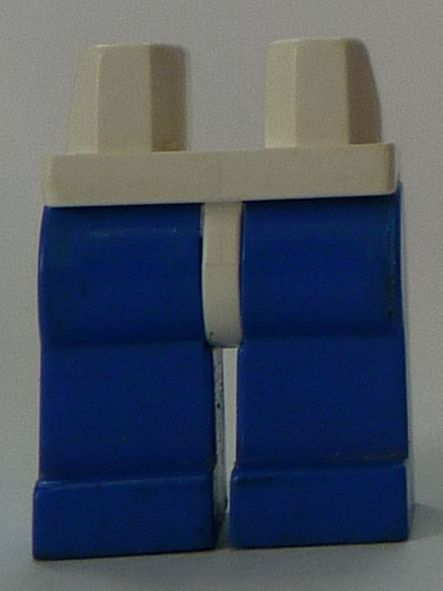
\includegraphics[width=.2\linewidth]{pants-blue}\hfill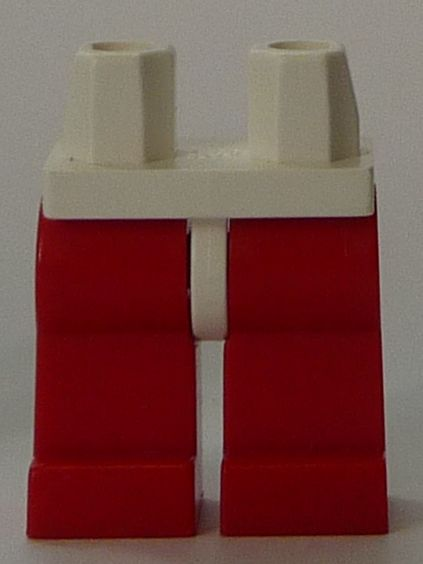
\includegraphics[width=.2\linewidth]{pants-red}\hfill~
		\end{example}

		\begin{example}{Cloning Whole Products (Clone-and-Own)}
			~\hfill
\includegraphics[width=.2\linewidth]{130}\hfill
\includegraphics[width=.2\linewidth]{230}\hfill~
		\end{example}
	\end{mycolumns}
}

% introduced: 02a-configuration
% reused: 03a-intro
\newcommand{\frameImplementSPLs}{
	\begin{mycolumns}[widths={45},animation=none]
		\pic[width=\linewidth]{metaproduct2}
	\mynextcolumn
		\begin{note}{Key Issues}
			\begin{itemize}
			\item Systematic reuse of implementation artifacts
			\item Explicit handling of variability
			\end{itemize}
		\end{note}
		\uncover<2->{\begin{definition}{Variability\mysource{\fospl\mypage{48}}}
			\mycite{\emph{Variability} is the ability to derive different products from a common set of artifacts.}
		\end{definition}}
		~
		\uncover<3->{\begin{note}{Variability-Intensive System}
			Any software product line is a variability-intensive system. % TODO Timo: do we really need this term? where does this definition come from?
		\end{note}}
	\end{mycolumns}
}

% introduced: 02a-configuration
% reused: 02b-implementation, 03a-intro
\newcommand{\frameVariabilityAndBindingTimes}{
	\begin{mycolumns}[widths={55},animation=none]
		\begin{definition}{Binding Time \deutsch{Bindungszeitpunkt}\mysource{\fospl\mypage{48}}}
			\begin{itemize}
				\item Variability offers choices
				\item Derivation of a product requires to make decisions (aka. binding)
				\item Decisions may be bound at different binding times
			\end{itemize}
		\end{definition}
		~
		\uncover<2->{\begin{note}{When? By whom? How?}
			\lectureruntime\parta: \emph{when} and \emph{by whom}

			\lectureruntime\partb: \emph{how}
		\end{note}}
	\mynextcolumn
		\pic[width=\linewidth]{metaproduct2}
	\end{mycolumns}
}

% introduced: 03a-intro
% reused: 03a-intro
\newcommand{\frameRuntimeVariabilityProblems}{
	\begin{note}{Problems of Runtime Variability}
		{\bf Conditional Statements:}
		\begin{itemize}
			\item Code scattering, tangling, and replication
		\end{itemize}
		{\bf Design Patterns for Variability:}
		\begin{itemize}
			\item Trade-offs and potential negative side effects
			\item Constraints that may restrict their usage
		\end{itemize}
		{\bf In General:}
		\begin{itemize}
			\item Variable parts are always delivered
			\item Not well-suited for compile-time binding
		\end{itemize}
	\end{note}
}

% introduced: 03a-intro
% reused: 03a-intro
\newcommand{\frameSoftwareConfigurationManagement}{
	\begin{mycolumns}
		\begin{definition}{Software Configuration Management} % TODO source missing
			Policies, processes, and tools for managing evolving software systems:
			\begin{itemize}
				\item \emph{Version control}
				\item \emph{System building}
				\item Release management
				\item Change management
				\item Collaborative work
			\end{itemize}
		\end{definition}
	\mynextcolumn
		\begin{note}{No Software Configuration Management}
			\lecturecloneandown\parta: Ad-Hoc Clone-and-Own

			aka.\ unmanaged clone-and-own
		\end{note}
		\begin{note}{Version Control}
			\lecturecloneandown\partb: Clone-and-Own with Version Control

			instance of managed clone-and-own
		\end{note}
		\begin{note}{System Building}
			\lecturecloneandown\partc: Clone-and-Own with Build Systems

			instance of managed clone-and-own
		\end{note}
	\end{mycolumns}
}
